% Conversion avec : convert -density 300 -flatten img.pdf img.png
\documentclass{standalone}
\usepackage{xcolor,pgf,tikz,tkz-tab,pgfplots,xfp}
\pgfplotsset{compat=1.15}
\usetikzlibrary{arrows,backgrounds,calc}
\begin{document}
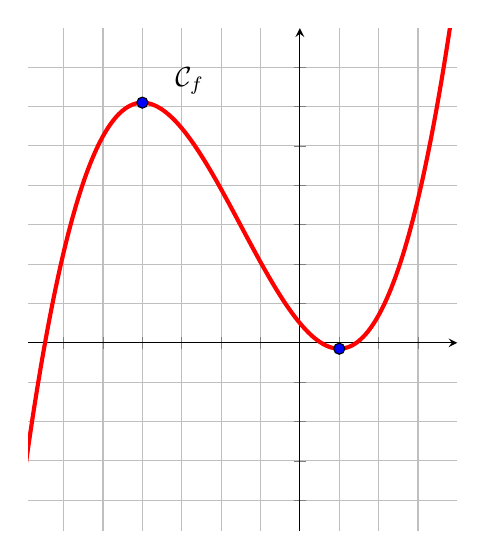
\begin{tikzpicture}
	\begin{axis}[x=0.5cm,y=0.05cm,axis lines=middle,ymajorgrids=true,xmajorgrids=true,xmin=-6.9,xmax=4,ymin=-47.9,ymax=79.9,xtick={-8.0,-7.0,...,3.0},ytick={-40.0,-30.0,...,80.0},yticklabel=\empty,xticklabel=\empty]
		\draw[line width=1.5pt,color=red,smooth,samples=100,domain=-7:4] plot(\x,{(\x)^(3.0)+4.5*(\x)^(2.0)-12*(\x)+5});
		\draw (-3.4116049405390774,72.3798051634355) node[anchor=north west] {$\mathcal{C}_f$};
		\draw [fill=blue] (-4,61) circle (2pt);
		\draw [fill=blue] (1,-1.5) circle (2pt);
	\end{axis}
\end{tikzpicture}
\end{document}
